\chapter{État de l'art du problème SMEPC}
\minitoc
\newpage
\label{Etat_art_probleme}
%regrouper les articles dans un tableau en mettant leurs caractéristiques
\section{Introduction}
Le problème de tournées de véhicules (en anglais \textit{Vehicle Routing Problem} et en abrégé VRP) est une classe de problème en recherche opérationnelle et en optimisation combinatoire. Cette classe de problème a été définie pour la première fois par Dantzig et Ramser en 1959 \cite{Dantzig_1959}. Les auteurs proposent une étude concernant la définition d'une flotte de véhicules qui fonctionnent au gasoil et qui fait des livraisons entre un client particulier et les autres clients. Les auteurs présentent un programme linéaire qui modélise ce problème dont l'objectif est de minimiser la distance parcourue par les véhicules. Dans cette classe de problème dans la plupart des cas on calcule les tournées d'un ensemble de véhicules afin de livrer une liste de clients désignés comme des stations. L'objectif est de servir ces clients en minimisant un ou plusieurs critères liés au coût de livraison des paquets. Ce problème est une extension classique du problème du voyageur de commerce. De nombreuses variantes du problème de tournées de véhicules sont survenues au fil des années, à l'instar du problème de tournées de véhicules avec contraintes de capacité (C-VRP) où les véhicules ont une capacité limitée (quantité, taille, poids, etc.), du problème de tournées de véhicules avec fenêtres de temps (VRP-TW) où pour chaque client on impose une fenêtre de temps dans laquelle la livraison doit être effectuée, ou encore du problème de tournées de véhicules avec collecte et livraison (PD-VRP) où un certain nombre de marchandises doivent être déplacées de sites de collecte vers des sites de livraisons, etc. Ce chapitre est consacré à l'état de l'art du problème \textbf{SMEPC}.

\section{Recherche Opérationelle et Énergie	}
 L'émergence des sources d'énergies renouvelables (photovoltaïque, éolienne, à base d'hydrogène ou de biomasse : (voir \cite{article_hydro_elect_hybrid2}, \cite{article_hydro_elect_hybrid1}, \cite{Grimes}, \cite{Licht2008})), qui visent à remplacer les gaz émetteurs de CO2 par de l'énergie électrique propre, ainsi que la rareté actuelle des infrastructures de charge/recharge connexes, ont suscité au cours des dernières décennies l'intérêt des chercheurs. La plupart des contributions ont porté sur les véhicules électriques ou hybrides nécessaires pour minimiser leur consommation d'énergie (problème de minimisation de la pollution et problème des véhicules hybrides : (voir \cite{article_GVRP3}, 	\cite{article_GVRP8}, \cite{article_GVRP10}, \cite{article_GVRP2}, \cite{article_GVRP13}, \cite{article_HVRP2}, 	\cite{article_GVRP16}). Des modèles connexes prennent en compte les transactions de recharge soumises à des fenêtres temporelles ou à des contraintes d'accès partagé (voir \cite{article_GVRP9}, \cite{article_GVRP4}, \cite{article_RVRP1}, \cite{article_HVRP4}). Certains auteurs ont également abordé la question de la programmation d'un processus industriel (voir \cite{Energy-Efficient-Albers-Susanne}, \cite{ANGEL20141}, \cite{inproceedings-Baptiste-Modeles}, \cite{quilliot:hal-01366540}, \cite{article-Demaine-Scheduling}, \cite{article_prod3}) tout en tenant compte des variations temporelles des coûts énergétiques, des restrictions d'accès et des préoccupations environnementales. Bien que la plupart des contributions aient été associées à des applications, il convient de mentionner l'existence de plusieurs contributions théoriques qui traitent des questions de complexité et d'approximation, pour des modèles qui mettent en jeu le coût de l'inactivité et l'impact des dépendances temporelles (voir \cite{Energy-Efficient-Albers-Susanne}, \cite{ANGEL20141}, \cite{quilliot:hal-01366540}, \cite{article-Homogeneously-alain}, \cite{article-Demaine-Scheduling}, \cite{article-Irani-Algorithmic}). D'autre part, les principaux producteurs d'énergie mènent depuis longtemps des études systématiques sur la manière de planifier la production d'énergie (gaz, électricité, gestion des barrages ou des centrales nucléaires), selon une approche à grande échelle, c'est-à-dire dans le but de répondre à des demandes agrégées incertaines à grande échelle (voir \cite{845896A-survey-of-design}, \cite{article_prod2}, \cite{article_prod1}, \cite{article_prod4}, \cite{RePEc:eee:ejores:v:261:y:2017:i:1:p:67-74}).

Dans cette section, on présentera d'abord les problèmes de tournées de véhicules qui mettent l'accent sur la gestion de l'énergie c'est-à-dire qui tiennent compte de l'alimentation des véhicules lors de la planification des tournées de véhicules. Ensuite, on fera un état de l'art des problèmes de production et enfin, on présentera des problèmes de la littérature qui jumellent planification de tournées de véhicules et production d'énergie à l'aide d'un mécanisme de synchronisation.

\subsection{Planification des tournées de véhicules et alimentation des véhicules}
%	Le problème de tournée de véhicule, en anglais Vehicle Routing Problem (VRP), est apparu pour la première fois en 
%Le problème de tournée de véhicule couplé 
Plusieurs auteurs ont traité des problèmes de tournées de véhicules qui mettent l'accent sur la gestion de l'énergie qui alimente les véhicules au cours des tournées. Ces problèmes appartenant à la classe de problème VRP sont appelés Electric VRP (EVRP), Green VRP (GVRP), Hydrogen VRP (HVRP), Recharging VRP (RVRP) (voir figure (\ref{Etat_art_recharge}). On s'intéresse à la façon dont les véhicules sont alimentés en énergie et à la façon dont on manage l'énergie contenue dans les véhicules. A cet effet, on s'intéresse à la planification des tournées de véhicules en tenant compte du fait que ces véhicules doivent se recharger en énergie pour pouvoir se déplacer. Dans la suite, on présente toutes ces classes de problèmes.
%d'une part et à synchronisation de le production d'énergie et de la consommation de cette énergie par les véhicules d'autre part.

\begin{figure}[H]
	\centerline{
		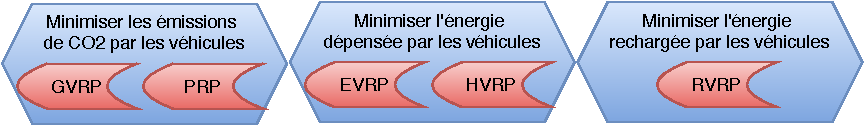
\includegraphics[height=2.5cm]{images_these/Etat_art_recharge.pdf}}
	\caption[Problèmes incluant tournée de véhicules et gestion de leurs alimentations]{Classes de problèmes qui incluent tournée de véhicules et gestion de leurs alimentations.}
	\label{Etat_art_recharge}
\end{figure}
\subsubsection{GVRP : \textit{Green Vehicle Routing Problem}}

Le terme \og logistique verte \fg{} définit un sujet qui a été intensément étudié (voir \cite{Alizadeh_Foroutan_2020} \cite{article_GVRP12} \cite{Antonio_2020} \cite{article_GVRP10} \cite{article_GVRP2} \cite{article_GVRP11} \cite{article_GVRP13} \cite{article_GVRP9} \cite{article_GVRP14} \cite{article_GVRP4} \cite{article_GVRP15} \cite{Ferani_2020}) et a attiré l'attention de nombreux professionnels de la recherche opérationnelle. La classe de problème \textit{Green Vehicle Routing Problem} (G-VRP) appartenant à la classe de problème VRP est alors apparue. G-VRP vise à minimiser les émissions de dioxyde de carbone (CO2) dans les systèmes logistiques grâce à une meilleure planification des livraisons effectuées par une flotte de véhicules. G-VRP a été énoncé pour la première fois par Sevgi Erdogan et Elise Miller-Hooks en 2012 dans l'article \cite{article_GVRP2}.

Le G-VRP est défini dans l'article \cite{article_GVRP11} sur un graphe complet orienté $G = (N, A)$, où $N = "0" \cup N_c \cup F$ est l'ensemble des nœuds et $A = \{(n_i, n_j):n_i, n_j, \in N\}$ est l'ensemble des arcs qui relient les nœuds dans $N$. La signification de l'ensemble des nœuds $N$ est la suivante :
\begin{itemize}
	\item $"0"$ correspond au dépôt ;
	\item $N_c= \{n_1, n_2, \dots, n_c\}$ est l'ensemble des nœuds clients et le nombre de client maximal est $c$ ;
	\item $F = \{n_{c+1}, n_{c+2}, \dots, n_{c+s}\}$ est l'ensemble des nœuds de recharge (aussi appelé station-service) et le nombre de stations de recharge maximal est $s$.
\end{itemize}
Un nombre illimité de véhicules homogènes est disponible au dépôt pour servir les clients avec une capacité de réservoir de carburant $Q$ (litres) et un taux de consommation de carburant $r$ (litres par kilomètre). Chaque véhicule se déplace sur le graphe $G$ à une vitesse constante $sp$ (kilomètres par heure). Chaque arc $(n_i, n_j) \in A$ est associé à une distance non négative $d_{ij}$, un temps de parcours $t_{ij}$ associé à la distance ($t_{ij}= d_{ij}/sp$).
% et également la distance respecte l'inégalité du triangle ($d_{ij}+ d_{jk} \geq d_{ik}$).
 Chaque nœud est associé à un temps de service $p_i$, qui représente le service.
Le dépôt peut servir de station-service et toutes les stations de carburant ont une capacité illimitée. Il n'y a pas de limite au nombre d'arrêts pour le ravitaillement en carburant et le réservoir du véhicule est supposé être plein après avoir quitté une station-service. Il existe un temps maximal ($Tmax$) qui fixe la durée d'une journée de travail et le problème est de déterminer les tournées des véhicules de manière à minimiser le coût total, en se basant sur les hypothèses suivantes : chaque véhicule est utilisé pour un itinéraire au maximum ; chaque itinéraire commence et se termine au dépôt ; le niveau de carburant dans le réservoir du véhicule doit être supérieur ou égal à la consommation de carburant entre deux nœuds quelconques ; la quantité de carburant dans le réservoir d'un véhicule est suffisante pour pouvoir circuler entre deux nœuds quelconques ; la durée de l'itinéraire attribué à un véhicule ne peut pas dépasser la durée maximale.

%Le problème \textit{Green Vehicle Routing Problem} (G-VRP) a été énoncé pour la première fois par Sevgi Erdogan et Elise Miller-Hooks en 2012
 Dans l'article \cite{article_GVRP2}, Sevgi Erdogan et Elise Miller-Hooks définissent le problème G-VRP. Dans leur définition, on a plusieurs stations de recharge et elles sont distinctes du dépôt. Ils proposent deux heuristiques : l'une basée sur l'algorithme de Clark et Wright et l'autre basée sur l'algorithme \textit{Density Based Clustering} (DBCA). Ils comparent leurs résultats à leur modèle linéaire du problème de G-VRP. Il en résulte que l'algorithme DBCA est meilleur que l'algorithme de Clark et Wright car il fournit de meilleures solutions. Les auteurs montrent que la faisabilité du problème dépend fortement de l'emplacement des stations et des stations de recharge. On minimise ici la distance parcourue par les véhicules.

Dans l'article \cite{article_GVRP9}, Marcos Raylan Sousa Matos et al. traite en 2018 le problème Green Vehicle Routing Problem (G-VRP). Dans ce document, le GVRSP prend en compte les véhicules hétérogènes, la congestion, et les contraintes de capacité. La livraison peut être fractionnée. Ils proposent un algorithme hybride qui combine une métaheuristique Iterated Local Search (ILS) et la procédure Random Variable Neighborhood Descent (RVND) En outre, ils utilisent un ensemble de couverture exact (SC), qui détermine la meilleure combinaison de tournées générés pendant l'exécution de l'ILS. Leur algorithme a permis de réduire le coût du CO2 dans les 140 instances testées par rapport aux résultats du GVRSP sans livraison fractionnée présentée dans \cite{Xiao_heterogeneous_2016}, tout en ayant un délai compétitif.

Dans l'article \cite{article_GVRP4}, Martin Sachenbacher et al. abordent le problème G-VRP de façon théorique en considérant les stations comme des sommets d'un graphe noté $G$, les routes qui relient les stations comme des arcs de $G$ et les tournées comme des chemins. Chaque arc est étiqueté par la quantité d'électricité qu'il faut à un véhicule électrique pour le parcourir. Ils calculent le plus court chemin entre deux sommets $u$ et $v$ du graphe $G$ en utilisant plusieurs algorithmes connus. Plus précisément, ils comparent en 2011 les résultats de l'algorithme Dijkstra et de l'algorithme $A^*$. Le plus court chemin entre deux sommets $u$ et $v$ est défini ici comme le chemin qui nécessite la plus petite quantité d'énergie au véhicule électrique pour se déplacer de $u$ à $v$. Il en ressort l'algorithme $A^*$ fournit de meilleurs résultats car il est le plus rapide.

Dans l'article \cite{article_GVRP10}, Imdat Kara et al. définit en 2007 un nouveau problème qu'ils appellent \textit{Energy Minimizing Vehicle Routing Problem} (EM-VRP). Ils définissent le problème C-VRP sur un graphe $G = (V,A)$ où $V = {0, 1, 2, . . ., n}$ est l'ensemble des nœuds (sommets), $0$ est le dépôt (origine, ville d'origine), et les autres nœuds sont des clients. L'ensemble $A = \{(i, j) : i, j \in V, i \ne j\}$ est un ensemble d'arcs (ou d'arêtes). Chaque client $i \in V-\{0\}$ est associé à une demande entière et positive $q_i$ et à chaque arc $(i, j)$ est associé un coût de déplacement $c_{ij}$ (qui peut être symétrique, asymétrique, déterministe, aléatoire, etc.). On a $m $ véhicules de capacité identique Q. Le C-VRP consiste à déterminer un ensemble de $m$ tournées de véhicules avec un coût minimum de telle sorte que : chaque tournée commence et se termine au dépôt, chaque client est visité par une unique tournée, et la demande de chaque tournée ne dépasse pas la capacité des véhicules $Q$. La C-VRP a été définie pour la première fois par Dantzig et Ramser en 1959 \cite{Dantzig_1959}. Dans cette étude, les auteurs ont utilisé la distance parcourue comme substitut de la fonction de coût. Depuis lors, le coût du voyage du nœud $i$ au nœud $j$, c'est-à-dire $c_{ij}$ , a généralement été considéré comme la distance entre ces nœuds. Les auteurs définissent une nouvelle fonction de calcul du coût pour le problème Capacited Vehicle Routing Problem (C-VRP) qui comprend la distance parcourue par le véhicule et la charge du véhicule sur chaque arc. Lorsqu'ils comparent les résultats obtenus sur CPLEX de C-VRP et EM-VRP, ils constatent que EM-VRP calcule des tournées qui minimisent l'énergie totale consommée par les véhicules.

Dans l'article \cite{article_GVRP11}, Çagri Koç et Ismail Karaoglan proposent en 2016 une méta-heuristique basée sur le recuit simulé pour calculer une borne supérieure du problème G-VRP. La borne inférieure est calculée avec l'algorithme \textit{branch-and-cut}. Les résultats des calculs montrent que 22 des 40 cas avec 20 clients peuvent être résolus de manière optimale en un temps de calcul raisonnable.

Dans l'article \cite{article_GVRP12}, Juho Andelmin et Enrico Bartolini proposent en 2017 un algorithme exact pour résoudre G-VRP. Ils modélisent le G-VRP comme un problème de partitionnement d'ensemble dans lequel les colonnes représentent les tournées possibles correspondant à des circuits simples dans un multigraphe. Chaque nœud du multigraphe représente un client et chaque arc entre deux clients représente un chemin à travers un ensemble de stations de recharge visitées par un véhicule lorsqu'il voyage directement entre les deux clients. Ils renforcent la formulation du partitionnement de l'ensemble en ajoutant des inégalités valides, y compris des coupes de parcours, et ils décrivent une méthode pour les séparer. Ils fournissent des résultats sur des instances montrant que l'algorithme peut résoudre de manière optimale des instances ayant jusqu'à environ 110 clients.

Dans l'article \cite{article_GVRP13}, Yiyo Kuo propose en 2010 un algorithme basé sur le recuit simulé pour résoudre le problème \textit{time-dependent vehicle routing problem}
(TDVRP). L'auteur calcule ici des tournées qui minimisent la consommation de carburant par les véhicules. Une évaluation expérimentale de la méthode proposée est effectuée. Les résultats montrent que la méthode proposée permet une amélioration de 24,61 \% de la consommation de carburant par rapport à la méthode basée sur la minimisation du temps de transport et une amélioration de 22,69 \% par rapport à la méthode basée sur la minimisation des distances de transport. De plus, un modèle est proposé pour calculer la consommation totale de carburant pour le problème TDVRP. Dans le modèle, la consommation de carburant prend en considération le poids du chargement des véhicules.


Dans l'article \cite{article_GVRP14}, Nur Normasari et al. proposent en 2019 un algorithme basé sur le recuit simulé pour résoudre le problème \textit{Capacitated Green Vehicle Routing Problem}(CG-VRP), qui est une extension du problème GVRP, caractérisé par l'objectif d'harmoniser les coûts environnementaux et économiques en mettant en œuvre des tournées efficaces. Ils formulent le modèle mathématique du problème et mettent en place un MIP. L'objectif du CGVRP est de minimiser la distance totale parcourue par un véhicule à carburant alternatif. Les résultats de l'expérience numérique montrent que l'algorithme est capable d'obtenir de bonnes solutions du CG-VRP dans un délai raisonnable, et l'analyse de sensibilité démontre que la distance totale dépend du nombre de clients et de l'autonomie du véhicule.

Dans l'article \cite{Alizadeh_Foroutan_2020}, Alizadeh Foroutan et al. proposent en 2020 un programme non-linéaire mixtes (MINLP) et deux méta-heuristiques basées sur le recuit simulé et l'algorithme génétique pour résoudre le problème G-VRP avec une flotte de véhicules hétérogènes. Il en résulte que l'algorithme basée sur le recuit simulé fournit de meilleurs solutions et l'algorithme génétique fournit des solutions plus rapidement sur des instances de grandes tailles dont le nombre de stations est 30.

Dans l'article \cite{article_GVRP15}, Yiyong Xiao et al. proposent en 2019 un programme linéaire à variables entières mixtes (MILP) et une heuristique basée sur la recherche à voisinage itératif (INS) appelé \textit{Dynamic Partial Optimization with Itterative Neighborhood Search} (DPO-INS) pour résoudre le problème \textit{Electric Vehicle Routing Problem With Time Windows considering Energy Consumption Rate} (EVRPTW-ECR). Dans EVRPTW-ECR, on veut planifier les tournées de véhicules en minimisant la distance parcourue, la vitesse de parcours et la quantité d'énergie électrique consommée au cours du parcours.
Les résultats démontrent que le MILP résout des instances jusqu'à 25 stations et l'heuristique résout des instances jusqu'à 100 stations.

%Dans l'article \cite{article_GVRP16}, Canhong Lin, et al. proposent en 2014

Dans l'article \cite{Antonio_2020}, Antonio Giallanza et Gabriella Li Puma proposent en 2020 une méta-heuristique basée sur l'algorithme génétique et un modèle de programmation par contrainte pour résoudre le problème \textit{three-echelon fuzzy green vehicle routing problem} abrégé 3E-FGVRP. Dans ce problème on veut mettre en place un \textit{agri-food supply chain} qui consiste à planifier le cycle suivant : la recherche de matière première, la production de marchandises, le stockage de marchandises, le transport de marchandises et la livraison de marchandises. Les auteurs font du mono-objectif en minimisant la somme de la distance parcourue par les véhicules, du coût de distribution de la marchandise et du coût d'émissions de carbone. Les auteurs réalisent une étude de cas de l'\textit{agri-food} Sicilien.

Dans l'article \cite{Ferani_2020}, Ferani E. Zulvia et al. proposent en 2020 un algorithme \textit{Many-Objective Gradient Evolution} (MOGE) basé sur l'algorithme \textit{gradient evolution} (GE) pour résoudre le problème GVRP avec fenêtre de temps. GE consiste à parcourir un espace de solutions à l'aide de trois opérations : la mise à jour, le saut et le rafraîchissement. Les véhicules sont utilisés pour le transport de produits périssables. L'objectif est de minimiser :
\begin{itemize}[label=$\square$]
	\item Le coût opérationnel qui est constitué du coût du carburant et du coût d'utilisation des véhicules ;
	\item Le coût de détérioration des produits ;
	\item Le coût d'émission de carbone ;
	\item Le coût de satisfaction des clients (respecter les fenêtres de temps attribuées à chaque client).
\end{itemize}


\subsubsection{PRP : \textit{Pollution-Routing Problem}}

%Le problème Pollution-Routing Problem (PRP) consiste à calculer les tournées de véhicules pour servir un ensemble de clients et à déterminer leurs vitesses sur chaque segment de route dans le but de minimiser les émissions de gaz à effet de serre. Les véhicules sont confrontés à des embouteillages qui, aux périodes de pointe, limitent considérablement leur vitesse et entraînent une augmentation des émissions de gaz à effet de serre.

Le \textit{Pollution-Routing Problem} (PRP) a été formulé pour la première fois en 2011 par Bektas et Laporte dans \cite{BEKTAS20111232}. Ce problème a été abordé dans plusieurs articles (voir \cite{article_GVRP7}, \cite{article_GVRP6}, \cite{article_GVRP8}, \cite{PRP_Franceschetti_2013}, \cite{PRP_Ko_2014}, \cite{PRP_Rui_2020}, \cite{PRP_Erfan_2020}, \cite{PRP_Yiyong_2020}). C'est un problème d'optimisation qui consiste à trouver un équilibre entre coût
monétaire et coût environnemental (émission de gaz à effet de serre) des entreprises de logistique qui livrent des clients avec des véhicules alimentés aux combustibles fossiles. Dans \cite{BEKTAS20111232}, les auteurs préspécifient un ensemble de vitesses que les véhicules peuvent prendre, ce qui conduit à des solutions sous-optimales car les temps de trajet sont discrétisés. Cette stratégie de discrétisation est aussi utilisée par Franceschetti et al. \cite{PRP_Franceschetti_2013} pour résoudre le \textit{Time-Dependent PRP} (TD-PRP), par Demir et al. \cite{article_GVRP6} pour résoudre le problème Bi-objective PRP et par Koc et al. \cite{PRP_Ko_2014} pour résoudre le problème Heterogeneous PRP.

Le problème PRP consiste à calculer les tournées de véhicules pour servir un ensemble de clients dans le but de minimiser les émissions de gaz à effet de serre. Les véhicules sont confrontés à des embouteillages
qui, aux périodes de pointe, limitent considérablement leurs vitesses et entraînent une augmentation des émissions de gaz à effet de serre.

Dans la littérature, PRP a été défini de plusieurs façons en fonction du critère à optimiser. D'après \cite{BEKTAS20111232}, on peut classifier ces définitions en quatre catégories à savoir les modèles minimisant les émissions de gaz à effet de serre en optimisant :
\begin{itemize}[label=$\square$]
	\item La charge des véhicules ;
	\item La vitesse des véhicules ;
	\item Simultanément la charge et la vitesse des véhicules ;
	\item La charge des véhicules tout en évitant les congestions.
\end{itemize}

Dans l'article \cite{article_GVRP7}, E. Demir et al. proposent en 2012 un algorithme ALNS qui résout le problème Pollution-Routing. La métaheuristique ALNS est une extension de l'heuristique Local Neighborhood Search (LNS) proposée pour la première fois par Shaw \cite{article_Shaw} en 1997, et basée sur l'idée de modifier une solution initiale au moyen d'opérateurs de destruction et de réparation. Si la nouvelle solution est meilleure que la meilleure solution actuelle, elle la remplace et sert d'entrée à l'itération suivante. La métaheuristique ALNS quant à elle a été proposée par Ropke et Pisinger \cite{article_Ropke} en 2006 pour résoudre des variantes du VRP. Plutôt que d'utiliser un grand voisinage comme dans le LNS, elle applique plusieurs opérateurs de retrait et d'insertion à une solution donnée. Les opérateurs d'insertion sont utilisés pour réparer une solution partiellement détruite en réintégrant les stations de la liste de retrait dans la solution. Ces opérateurs réintègrent les stations supprimés dans les tournées existantes lorsque la faisabilité en termes de capacité et de délais peut être maintenue, ou ils créent de nouvelles tournées. Le voisinage d'une solution est obtenue en retirant certains stations de la solution et en les réintégrant d'une autre façon.


Dans l'article \cite{article_GVRP6} les auteurs proposent en 2013 un algorithme ALNS qui résout le \textit{Bi-objective Pollution-Routing Problem} qui est une extension du problème \textit{Pollution-Routing Problem} (PRP). Dans le \textit{Bi-objective Pollution-Routing Problem}, on a deux objectifs : l'un est de minimiser l'énergie consommé par les véhicules et l'autre est de minimiser la distance parcourue par les véhicules.


Dans l'article \cite{article_GVRP8}, Anna Franceschetti et al. proposent en 2017 une métaheuristique pour le problème \textit{Time-Dependent Pollution-Routing}. Ici, on minimise aussi le coût du salaire du conducteur.
Leur algorithme est basé sur une heuristique ALNS et utilise de nouveaux opérateurs de retrait et d'insertion qui améliorent considérablement la qualité de la solution. Une procédure d'optimisation des heures de départ et de la vitesse des véhicules, mise au point antérieurement, est utilisée comme sous-programme pour optimiser les heures de départ et la vitesse des véhicules. Les auteurs comparent les résultats obtenues par l'ALNS avec les résultats de CPLEX.

Dans l'article \cite{PRP_Yiyong_2020}, Yiyong et al. proposent en 2020 un \textit{$\epsilon$-accurate mixed integer linear program} pour résoudre le problème \textit{continuous PRP}. Ici les variables à optimiser peuvent prendre tout un continuum de valeurs. Le coefficient $\epsilon$ est le pourcentage d'erreur maximal admissible dans la linéarisation des relations entre le temps , la vitesse et la consommation de carburant. Les auteurs minimisent le temps de trajet des véhicules et la quantité de carburant consommée par les véhicules. Les expérimentations ont montré que le modèle $\epsilon$-CPRP pouvait donner de bonnes solutions.% que les modèles PRP discrets suivant : Demir et al. [6], Kramer et al. [28] et Fukasawa et al. [16].
  De plus, de nombreuses instances $UK\_PRP$ ont été mises à jour avec de nouvelles meilleures solutions.

%Dans l'article \cite{PRP_Rui_2020}, Rui et al. proposent en 2020

 Dans l'article \cite{PRP_Rui_2020}, Rui et al. définissent en 2020 un nouveau variant du problème PRP qu'ils appellent \textit{carbon pricing initiatives-based bi-level pollution routing problem} (CPIBPRP). Les gouvernements ont fixé des prix du carbone afin que les entreprises diminuent leurs émissions de carbone. Autrement dit, plus une entreprise produira du carbone, plus la taxe qu'elle devra payer sera élevée. CPIBPRP cherche à programmer les tournées de véhicules et on a deux objectifs à atteindre. Premièrement, on minimise les émissions de carbone et, deuxièmement, on doit respecter les limites imposées par le gouvernement concernant la quantité de carbone à produire. Les auteurs définissent d'abord un modèle à deux niveaux pour CPIBPRP. Ensuite, pour résoudre ce problème les auteurs développent un algorithme interactif intégrant l'optimisation par essaims de particules contrôlée par la logique floue et une heuristique ALNS modifiée. Ils le nomment \textit{algorithm integrating fuzzy logic controlled particle swarm optimization (FLCPSO) and the modified ALNS heuristic} (IFLCPSO-MALNS). Les résultats montrent que l'application des initiatives de tarification du carbone peut réduire les émissions de carbone en augmentant relativement peu le coût total des entreprises de transports de marchandises.


%Dans l'article \cite{PRP_Erfan_2020}, Erfan et al. proposent en 2020
Dans l'article \cite{PRP_Erfan_2020}, Erfan et al. définissent en 2020 un variant du problème PRP qu'ils appellent \textit{Pollution-Routing Problem with Cross-dock Selection} (PRP-CDS).
Le cross docking est une méthode d'expédition très utilisée pour simultanément réduire les coûts de stockage, transporter la marchandise des fournisseurs aux clients le plus rapidement possible et minimiser les dommages causés à la marchandise. Cette méthode se déroule en trois étapes :
\begin{enumerate}
	
\item On reçoit la marchandise dans les entrepôts de cross docking ;
 \item On décharge la marchandise, on la vérifie et on la trie en fonction de sa destination ;
\item On expédie la marchandise aux clients le plus rapidement possible.
\end{enumerate}
PRP-CDS consiste à planifier le trajet des véhicules en visant deux objectifs :

\begin{itemize}[label=$\square$]

\item Premièrement, minimiser le coût de pollution et le coût de transport des marchandises. Ici les conditions du trafic et la vitesse des véhicules déterminent la consommation de carburant et la pollution ;
\item Deuxièmement, maximiser la satisfaction des clients liée à la quantité moyenne de marchandises transportés vers les entrepôts de cross docking.
\end{itemize}
Pour résoudre le problème PRP-CDS, les auteurs développent une méthode exacte \textit{Bi-Objective Mixed Integer Linear Programming} (BOMILP) et deux métaheuristiques dont l'une est basée sur le \textit{Multi-Objective Simulated-annealing Algorithm} (MOSA) et l'autre est basée sur le \textit{Non-dominated Sorting Genetic Algorithm II} (NSGA-II). Après la phase expérimentale, il en ressort que les algorithmes proposés fournissent de bonnes solutions et que c'est l'algorithme NSGA-II qui est le plus efficace.


\subsubsection{EVRP : \textit{Electric Vehicle Routing Problem}}
Les véhicules électriques sont une nouvelle génération de véhicules qui fonctionnent à l'aide de batteries. Le durée de recharge d'une batterie est longue, raison pour laquelle les modèles et algorithmes de VRP classique ne sont pas adaptés pour planifier les trajets de ces véhicules, d'ou l'apparition de la classe de problèmes Electric VRP (E-VRP). De nombreux auteurs ont conçu des modèles et algorithmes pour traiter les problèmes E-VRP (voir \cite{EVRP_Sina_2020}, \cite{EVRP_Rui_2020}, \cite{article_GVRP3}, \cite{EVRP_Rasoul_2020}, \cite{EVRP_Surendra_2020}, \cite{EVRP_Kexing_2020}, \cite{EVRP_Ji_2020}, \cite{article_RVRP1}, \cite{article_HVRP4}, \cite{EVRP_Shuai_2020}, \cite{article_GVRP1}).

Dans l'article \cite{article_GVRP1}, Shuai Zhang et al. proposent en 2018 une méta-heuristique basée sur l'algorithme Colonie de Fourmis (dont les perturbations sont effectuées par Iterated Local Search) pour résoudre E-VRP. On a ici plusieurs stations de recharge dont le dépôt ne fait pas partie. Ils montrent qu'utiliser l'énergie consommée par les véhicules comme fonction objectif donnent de meilleurs solutions que de considérer la distance comme fonction objectif. Ils ont implémenté un algorithme Adaptative \textit{Local Neighborhood Search} (ALNS) et un modèle linéaire qu'ils comparent avec la méta-heuristique. Ils en ressort que la méta-heuristique est meilleure que l'algorithme ALNS car il fournit de meilleurs solutions plus rapidement. 


Dans l'article \cite{article_GVRP3}, Çagri Koç et al. veulent calculer à quels endroits seront placés les stations de recharge et quelle technologie (vitesse de recharge rapide, moyenne ou lente) de recharge devra être affectée à chaque station. Ce problème est appelé dans la littérature E-VRP \textit{with shared charging stations} (E-VRP-SCS). Ici, les stations de recharge et le dépôt sont distincts. Pour résoudre le problème E-VRP-SCS, ils proposent en 2018 une heuristique ALNS comprenant des étapes d'intensification et de diversification de la solution réalisées par des opérateurs d'insertion et de suppression de stations. La fonction coût est constituée du coût de la tournée et du coût de l'ouverture des stations. Ils ont comparé l'heuristique ALNS à un modèle linéaire MIP.

Dans l'article \cite{article_RVRP1}, Michael Schneider et al. traitent en 2014 le problème \textit{Electric Vehicle Routing Problem with Time Windows} (E-VRPTW) en tenant compte des recharges en électricité des véhicules. Chaque station a une fenêtre temporelle et un temps de service. Le service ne peut pas commencer avant la date de début de la fenêtre temporelle, ce qui peut entraîner un temps d'attente, et ne peut pas commencer après la date de fin de la fenêtre temporelle. Pour résoudre le problème E-VRPTW, ils conçoivent une heuristique basée sur une combinaison de l'algorithme de recherche à voisinage variable (\textit{Variable Neighborhood Search}) et de la recherche tabou (\textit{Tabou Search} en anglais). Ils démontrent l'efficacité de cette heuristique en la comparant avec une formulation linéaire implémenté sur CPLEX. 

Dans l'article \cite{EVRP_Ji_2020}, Ji et al. définissent en 2020 un nouveau problème appelé \textit{Time-dependent Electric Vehicle Routing Problem} (TDEVRP). L'objectif de ce problème est de planifier le trajet des véhicules électriques en tenant compte de périodes de congestion qui correspondent à des heures de pointe fixées le matin et le soir chaque jour. On tient aussi compte des décisions de recharge des véhicules qui ont lieu aux stations. On tient aussi compte ici de la quantité d'énergie consommée par les véhicules : celle-ci est calculée grâce aux poids préalablement fixés sur les routes, à la vitesse des véhicules et à la distance des routes. Pour résoudre le problème TDEVRP, ils définissent un programme linéaire en nombres entiers et un algorithme basé sur la recherche à voisinage variable. Cet algorithme fournit d'excellents résultats pour des instances de petites tailles (pas plus de 15 stations) et il fournit un gap en moyenne de 2,38\% pour des instances de grandes tailles. 

Dans l'article \cite{EVRP_Rui_2020}, Rui et al. proposent en 2019  un modélisation mathématique à deux niveaux (en anglais bi-level programming problem) du problème E-VRP-SCS. Ce modèle calcule la localisation et la capacité des stations de recharge pour des véhicules électriques. La programmation mathématique à deux niveaux résout des problèmes dont la structure hiérarchique est constituée de deux unités de prise de décision. Ici, on modélise la situation de plusieurs décideurs qui veulent réaliser leurs objectifs respectifs mais ne peuvent le faire indépendamment les uns des autres. Le problème de niveau supérieur minimise le coût de construction des installations de recharge et le coût de transport des marchandises. Le problème de niveau inférieur capture les réponses des conducteurs des véhicules aux décisions du niveau supérieur. Au cours des expérimentations du modèle, les auteurs évaluent les performances du modèle, la robustesse des solutions et l'évolutivité des solutions sur de grands réseaux.  


%Dans l'article \cite{EVRP_Rasoul_2020}, Rasoul et al. proposent en 2020
Dans l'article \cite{EVRP_Rasoul_2020}, Rasoul et al. proposent en 2020 un framework basé sur la théorie des jeux pour résoudre le problème de routage intelligent des véhicules électriques pour l'équilibrage des charges dans un réseau intelligent. Pour cela, ils tiennent compte des embouteillages et du temps d'attente des véhicules aux stations de recharge. Le problème EVRP est formulé ici comme un jeu non coopératif répété.  Si on a un ensemble de joueurs qui joue à un jeu dans lequel chacun cherche à optimiser ses gains, on aura un équilibre de Nash si chaque joueur a une stratégie tel qu'aucun ne peut obtenir un gain supplémentaire en changeant unilatéralement de stratégie. L'équilibre de Nash renvoie à un critère d'absence de regret. Il est montré dans cet article que tout équilibre de Nash obtenu améliore sensiblement l'équilibrage des charges sur le réseau.

La vulgarisation du télétravail a fait naitre de nouvelles problématiques. Certains propriétaires de véhicules électriques aimeraient partager leurs véhicules de manière rentable tout en s'assurant des heures de travail suffisantes sur un poste de travail à domicile. Dans l'article \cite{EVRP_Kexing_2020}, Kexing et al. proposent en 2020 un modèle permettant à ces propriétaires de pouvoir faire une planification optimale en minimisant simultanément le coût de recharge de leurs véhicules et le temps de livraison des clients. Le véhicule a trois états possibles : soit il est en charge, soit il est sur le parkings, soit il est entrain de transporter des clients. Les actions du propriétaire permettent de faire passer le véhicule d'un état à un autre. Les résultats numériques obtenus avec CPLEX démontrent l'efficacité de ce modèle.

Dans l'article \cite{EVRP_Surendra_2020}, Surendra et al. proposent en 2020 un modèle pour le problème E-VRP \textit{with Non-Linear charging and Load-Dependent discharging} abrégé E-VRP-NL-LD. Dans ce problème, on a une flotte illimité de véhicules électriques homogènes dont la capacité de recharge est fixée à $Q$ kWh. Cette flotte est chargée de réaliser des tâches de livraison à un ensemble de clients. Pour pouvoir se déplacer, au cours de leurs parcours, ces véhicules vont se recharger en électricité dans des stations de recharge préalablement fixées. Les véhicules commencent leurs tournées dans une station particulière appelée ici dépôt. Les véhicules ont un temps maximal Tmax pour finir leurs tournées. On veut minimiser la durée des trajets qui inclut aussi la durée des recharges. Les auteurs proposent aussi un algorithme ALNS pour résoudre ce problème. Les expérimentations numériques montrent que l'ALNS améliore les algorithmes existants pour 63\% des instances et obtient la solution optimale pour 31\% des instances.
 
Dans l'article \cite{EVRP_Shuai_2020}, Shuai et al. proposent en 2020 un modèle d'optimisation floue du problème \textit{electric vehicle routing problem with time windows and recharging stations} abrégé EVRPTW. Un algorithme ALNS y est aussi proposé pour résoudre ce modèle.

Dans l'article \cite{article_HVRP4}, Rashid Waraich et al. proposent en 2014 un modèle de simulation à événements discrets multi-agents afin d'obtenir un modèle de la dépendance temporelle des demandes et des coûts par rapport à une flotte de véhicules électriques. 


\subsubsection{HVRP : \textit{Hydrogen Vehicle Routing Problem}}


Dans l'article \cite{article_HVRP1}, Simona Mancini propose en 2017 un \textit{Mixed Integer Linear Programming
} du problème \textit{Hydrogen Vehicle Routing Problem}. Afin de résoudre ce problème, elle propose aussi une méta-heuristique basée sur la recherche à voisinage large.
Le problème HVRP consiste à visiter un ensemble de clients en partant d'un dépôt. La flotte disponible est composée d'un nombre fixe de véhicules identiques. Puisque les tournées multiples ne sont pas autorisées, au plus un nombre de tournées correspondant au nombre de véhicules peuvent être planifiées. Chaque véhicule doit commencer et terminer sa tournée au dépôt. Chaque client est caractérisé par un temps de service donné. Chaque paire de clients est associée à un temps de déplacement et à une distance. Les vitesses de déplacement
sont supposées être constantes sur une route. En outre, aucune limite n'est fixée sur le nombre d'arrêts qui peuvent être effectués pour la recharge, mais chaque station de recharge ne peut être visitée qu'une seule fois. Lorsqu'une recharge est entreprise, on suppose que le réservoir est rempli à pleine capacité. Les tournées commencent et se terminent au dépôt et doivent contenir des visites aux stations de recharge, si elles sont nécessaires. Chaque trajet peut être parcouru en utilisant uniquement le moteur électrique ou le carburant. Un coût de pénalité supplémentaire est ajouté lorsque le carburant est utilisé afin de dissuader l'utilisation de ce mode et de promouvoir l'utilisation du moteur électrique. Une limite à la durée des tournées est imposée. De nombreux articles traitent ce problème (voir \cite{EVRP_Sina_2020} \cite{article_HVRP2}, \cite{article_HVRP1},  \cite{article_HVRP5}, \cite{article_HVRP3}).

Dans l'article \cite{EVRP_Sina_2020}, Sina et al. proposent en 2020 un algorithme exact de \textit{branch-and-price} et une heuristique pour résoudre le problème \textit{Plugin Hybrid Electric Vehicle} abrégé PHEV. Dans ce problème, on a un ensemble de véhicules qui fonctionnent avec de l'électricité et de l'essence. Ces véhicules doivent réaliser des tâches chez des clients. On veut minimiser la consommation totale d'énergie en utilisant les deux sources d'énergie de façon optimale. Les auteurs montrent que l'heuristique devient plus rapide lorsque la capacité de la batterie est plus importante. Ils présentent aussi une étude de cas sur la ville de Toronto et montrent que les véhicules utilisent de l'électricité dans les zones congestionnées du centre-ville et de l'essence dans les autres zones.

Dans l'article \cite{article_HVRP2}, Antti Lajunen fait en 2014 des simulations afin de réaliser une analyse coût-bénéfice. Cette analyse consiste à étudier la consommation d'énergie et les émissions de CO2 de 4 véhicules hybrides et un véhicule électrique. De cette étude il en ressort que les coûts d'investissement et de stockage sont les plus importants. De plus, ces types de véhicules permettent de réduire les émissions de CO2 et la consommation d'énergie.
 
Dans l'article \cite{article_HVRP5}, Vincent Yu, et al. définissent en 2016 le problème Hybrid VRP. Ils donnent une formulation mathématique de ce problème et ils proposent une heuristique basée sur le recuit simulé. Ils montrent que l'heuristique proposée fournit une solution au problème HVRP. 

Dans l'article \cite{article_HVRP3}, Lu Zhen et al. proposent en 2019 un nouveau variant du problème Hybrid VRP appelé HVRP avec mode de sélection. Ici on a un dispositif qui permet de selectionner la source d'énergie utilisée (l'électricité ou le carburant) lors des trajets.Les auteurs proposent une formulation mathématique de ce problème.



\subsubsection{RVRP : \textit{Recharging Vehicle Routing Problem}}

%Dans l'article \cite{article_Conrad}, 
Conrad et Figliozzi ont défini en 2011 un nouveau problème  appelé \textit{Recharging Vehicle Routing Problem} abrégé RVRP (voir \cite{ANGEL20141}, \cite{Energy-Efficient-Albers-Susanne}) avec des fenêtres de temps, où les véhicules ayant une autonomie limitée peuvent être rechargés chez les clients pendant le processus de service. Le RVRP constitue la base de l'EVRP dans lequel les fenêtres de temps des clients sont prises en compte et le temps de recharge est fixe. Pour traiter le RVRP, un algorithme itératif de construction et d'amélioration d'itinéraire a été utilisé.
% Plusieurs articles traitent ce problème (voir \cite{ANGEL20141}, \cite{Energy-Efficient-Albers-Susanne}).

%Dans l'article \cite{ANGEL20141}, Eric Angel et al. proposent en 2014

%Dans l'article \cite{Energy-Efficient-Albers-Susanne}, Albers Susanne propose en 2010	

Dans la section suivante, on donne juste quelques références qui traitent le problème de planification de la production. Nous ne nous attarderons pas sur ce problème car c'est un problème qui a été largement étudié dans la littérature. 
\subsection{Planification de la production}

La gestion de la production vise à planifier et contrôler la transformation des matières en produits fini. Elle implique la combinaison de ressources, parmi lesquelles les moyens matériels (les machines), les moyens humains (le personnel par qualification) et les matières (matières premières, matières consommables) dans un planning avec pour but d'assurer la fabrication du produit en qualité et en quantité définies. Dans un environnement économique devenu aussi concurrentiel que le notre, les enjeux financiers sont cruciaux. Le prix de vente des produits dépend de plus en plus de la demande du marché et reste très influencé par la concurrence. Afin de rester compétitive et surtout garantir une marge bénéficiaire convenable sur la vente de leurs produits, les entreprises industrielles ont pour principal recours la réduction du coût de production. Le champ d'action de la gestion de la production dans l'entreprise est vaste, couvre de nombreuses activités et interpelle les professionnels de différents domaines de formation.


Les contraintes rencontrées sont de divers ordres :
\begin{itemize}[label=$\square$]%,leftmargin=*
		
	\item Financières (produire à un coût optimal), coût des matières et consommables, coût de stockage des encours et des produits semi ouvrés, coût de gestion des magasins, coût des heures de travail supplémentaires, coût des arrêts faisant partie intégrante du coût de revient. Maîtriser ces derniers est aussi une garantie pour la commercialisation des produits finis. 
	
	\item Temporelles (produire dans les délais, assurer une livraison juste à temps). Il s'agit d'éviter les ruptures de stocks, éviter le gonflage des stocks de produits finis. Car cela a une incidence directe sur la satisfaction de la clientèle (pertes de commandes) ou sur la partie du coût de revient des produits finis dûe aux coûts supplémentaires du stockage. 
	
	\item Mécaniques (maintenance préventives et gestion des temps d'arrêt). Il s'agit d'anticiper sur les pannes et de prévoir des solutions alternatives en cas d'arrêt d'une machine. 
	
	\item Qualité (produire avec le moins de défauts possible, le moins de déchets) : un produit de bonne qualité participe à la fidélisation de la clientèle et véhicule l'image de marque de l'entreprise. 
	
	\item Planification, il s'agit d'assurer une circulation continue des flux, de détecter et de supprimer les goulets d'étranglement dans le circuit de production. Il s'agit donc aussi de définir un plan de production, de définir les gammes opératoires, d'ordonnancer les opérations, et enfin de gérer la répartition des taches durant tout le processus de fabrication.
	
\end{itemize}
On se focalise principalement sur l'état de l'art des méthodes de planification de la production. Il existe plusieurs types de plans de production :
\begin{itemize}[label=$\square$]
	
\item Le plan de production à court terme peut être vu comme une version détaillée et désagrégée du plan de production à moyen terme: il désagrège les familles de produits en articles individuels et il planifie la production sur un horizon plus court en tenant compte d'une découpe plus fine du temps en sous-périodes. 

\item La planification à moyen terme prend place dans un cadre de décision où le portefeuille de produits  et  le  processus  de  production  peuvent  être  considérés  comme  des  donnés irrévocables, fixées par la stratégie de l'entreprise. Les questions qui se posent à ce niveau de décision tactique portent donc sur l'utilisation optimale du système productif dans le but de satisfaire la demande prévisionnelle sur l'horizon du plan. 

\item Dans le très court terme, le département production se trouve confronté à une collection d'ordres de fabrication (OF) à exécuter. Chaque OF consiste en une liste d'opérations à effectuer, mais ne précise pas nécessairement l'ordre dans lequel ces opérations doivent être exécutées, ni l'instant auquel elles doivent être entamées, ni les postes de production auxquels elles doivent être affectées. Ordonnancer la production, c'est planifier les dates de lancement et de fin des opérations ainsi que l'affectation de ces opérations aux différents postes de production  susceptibles  de  les  exécuter.  On  classe  généralement  la  fonction d'ordonnancement parmi les activités de planification à très court terme, quoique dans le cas de l'ordonnancement de projets elle puisse parfois tenir compte d'un horizon de plusieurs années.
\end{itemize}

La planification de la production est un problème qui a été longuement étudié au fil des années (Voir \cite{PPP_Samir_2010}, \cite{PPP_Dmitry_2017}, \cite{RePEc:eee:ejores:v:261:y:2017:i:1:p:67-74}, \cite{845896A-survey-of-design}, \cite{PPP_Sandeep_2018}, \cite{PPP_Weiwei_2018}, \cite{PPP_Doga_2020}, \cite{PPP_Dev}, \cite{PPP_Saman_2016}, \cite{PPP_Yuvraj_2015}, \cite{PPP_Fanny_2016}, \cite{article-Irani-Algorithmic}, \cite{PPP_Kuttner_2009}, \cite{PPP_Yan_2009}, \cite{PPP_Yanfei_2010}, \cite{PPP_Jingran_2019}, \cite{PPP_Esmaeil_2018}, \cite{article_prod2}, \cite{article_prod1}, \cite{article_prod3}, \cite{article_prod4}, \cite{quilliot:hal-01366540}, \cite{article-Homogeneously-alain}, \cite{PPP_Lixin_2012}, \cite{PPP_Nicolas_2019}, \cite{PPP_Guisen_2020}, \cite{PPP_Hui_2019}).


Dans l'article \cite{article_prod3}, Haouassi Mustapha et al. programment en 2016 un processus de production industrielle soumis à un coût électrique linéaire à la pièce. Ils implémentent des modèles MILP et des algorithmes de programmation dynamique.

Dans l'article \cite{article_prod4}, Agnes Pechmann et Schöler se concentrent en 2011 sur la gestion des processus de consommation d'énergie qui impliquent des pics et des ruptures, comme dans l'industrie sidérurgique ou à l'intérieur de grands bâtiments.




%A faire debut

%Dans l'article \cite{PPP_Weiwei_2018}, Weiwei et al. proposent en 2018
%
%Dans l'article \cite{PPP_Kuttner_2009}, Kuttner et al. proposent en 2009
%
%Dans l'article \cite{PPP_Esmaeil_2018}, Esmaeil et al. proposent en 2018
%
%Dans l'article \cite{PPP_Lixin_2012}, Lixin et al. proposent en 2012
%
%Dans l'article \cite{PPP_Yan_2009}, Yan et al. proposent en 2009
%
%Dans l'article	\cite{PPP_Nicolas_2019}, Nicolas et al. proposent en 2019
%
%Dans l'article \cite{PPP_Sandeep_2018}, Sandeep et al. proposent en 2018
%
%Dans l'article \cite{PPP_Jingran_2019}, Jingran et al. proposent en 2019
%
%Dans l'article \cite{PPP_Saman_2016}, Saman et al. proposent en 2016
%
%Dans l'article \cite{PPP_Dev}, Devyaterikova et al. proposent en 2009
%
%Dans l'article \cite{PPP_Fanny_2016}, Fanny et al. proposent en 2016
%
%Dans l'article \cite{PPP_Yuvraj_2015}, Yuvraj et al. proposent en 2015
%
%Dans l'article \cite{PPP_Yanfei_2010}, Yanfei et al. proposent en 2010
%
%Dans l'article \cite{PPP_Hui_2019}, Hui et al. proposent en 2019
%
%Dans l'article \cite{PPP_Doga_2020}, Doga et al. proposent en 2020
%
%Dans l'article \cite{PPP_Guisen_2020}, Guisen et al. proposent en 2020
%
%Dans l'article \cite{PPP_Samir_2010}, Samir et al. proposent en 2020
%%%production planing problem
%
%%%Dans l'article \cite{PPP_Dev},
%
%
%Dans l'article	\cite{article_prod1}, Joon-Yung et al. proposent en 2013
%
%Dans l'article \cite{article_prod2}, Joon-Yung Moon and Jin-Woo Park proposent en 2013
%
%
%Dans l'article \cite{845896A-survey-of-design}, L. Benini et al. proposent en 2000
%
%Dans l'article \cite{quilliot:hal-01366540}, Alain Quilliot et al. proposent en 2013
%
%Dans l'article \cite{RePEc:eee:ejores:v:261:y:2017:i:1:p:67-74}, Pascale Bendotti et al. proposent en 2017
%
%Dans l'article \cite{article-Homogeneously-alain}, Alain Quilliot et al. proposent en 2011
%
%Dans l'article \cite{article-Irani-Algorithmic}, Sandy Irani et al. proposent en 2005
%
%Dans l'article \cite{PPP_Dmitry_2017}, Dmitry et al. proposent en 2017
%
%
%A faire fin







%*************\subsubsection{Planification de production avec prise en compte de coût énergétique}
%%\subsubsection{ Production discontinue}
%***********************\subsubsection{ Planification de production avec recyclage de l'énergie (cogénération)}
%
%\subsubsection{Ordonnancement de la production}
%*********************\subsubsection{Planification et contrôle de production d'énergie}%(Electrique)

%
%\subsubsection{ Calibrer volume de production par rapport aux besoins}
%\subsubsection{ Calibrer volume de production par rapport aux besoins}
%******************\subsubsection{Problème Resource-Constrained Project Scheduling Problem}

%Dans l'article \cite{PPP_Dmitry_2017}, Dmitry et al. proposent en 2017
%\section{Synchronisation production/consommation}
%\subsection{Problématique générale de synchronisation}
%\subsubsection{Synchronisation discrète}


\section{Problématique générale de synchronisation}
%Dans cette partie, nous expliquerons deux grands types de synchronisation à savoir la synchronisation discrète la synchronisation continue.
%\subsection{Synchronisation discrète}

La synchronisation a été longuement étudiée dans la littérature (Voir \cite{article_synchro2}, \cite{article_synchro1}, \cite{article_synchro3}, \cite{IRP_Adulyasak}, \cite{IRP_Alvarez_2019}, \cite{IRP_Alvarez}, \cite{IRP_Archetti_2012}, \cite{IRP_Archetti}, \cite{IRP_Archetti_2017}, \cite{IRP_Chitsaz}, \cite{IRP_Leandro}, \cite{IRP_Coelho_2014}, \cite{IRP_Guy}, \cite{article_GVRP5}, \cite{IRP_Hewitt}, \cite{PRP_Panagiotis_2020}, \cite{IRP_Edcarllos}).

%\cite{article-Demaine-Scheduling},\cite{inproceedings-Baptiste-Modeles} \cite{inproceedings-Baptiste-Scheduling}, 
Dans l'article \cite{article_synchro1}, Martin Fink et al. traitent en 2019 le problème \textit{abstract vehicle routing problem with worker and vehicle synchronization} abrégé AVRPWVS. Ici, les auteurs cherchent à planifier la manutention au sol dans un aéroport. Les opérations planifiées sont par exemple le ravitaillement des avions et le déchargement des bagages. Pour réaliser ces tâches, Les employés doivent se déplacer d'un endroit à un autre dans l'aéroport avec des véhicules. Pour résoudre AVRPWVS, les auteurs développent un modèle mathématique et une heuristique basée sur le Branch and Price.

Dans l'article \cite{article_synchro2}, Michael Drexl fait en 2012 un état de l'art du problème Vehicle Routing Problem with Multiple Synchronization Constraints dont l'acronyme est VRPMS. L'auteur présente d'abord une classification des différents types de synchronisation à savoir la synchronisation de charge, la synchronisation de ressources, la synchronisation d'opérations et la synchronisation de mouvements. Puis, Il analyse ensuite des questions centrales liées aux solutions exactes et heuristiques de ces problèmes. Il passe enfin en revue de manière exhaustive la littérature pertinente en ce qui concerne les applications et les approches de résolution.

Dans l'article \cite{article_synchro3}, Ran LIU et al. proposent en 2018 une heuristique \textit{Atadaptive Large Neighborhood Search} pour résoudre le problème \textit{Vehicle Routing Problem With Time Windows and Synchronized Visits}
(un problème de routage de véhicules avec des fenêtres de temps et des visites synchronisées).
Des méthodes efficaces d'évaluation des solutions et de vérification de la synchronisation croisée y sont proposées. L'efficacité de l'approche y est ensuite prouvée.

%Dans l'article \cite{article-Demaine-Scheduling}, Erik Demaine et al. proposent en 2007

%Dans l'article \cite{inproceedings-Baptiste-Scheduling}, Philippe Baptiste proposent en 2006

%Dans l'article \cite{inproceedings-Baptiste-Modeles}, F. Sourd et al. proposent en 2004

%\subsection{Synchronisation continue : IRP / MIRP / extensions MIRP}

%La synchronisation a été longuement étudiée dans la littérature (Voir \cite{IRP_Adulyasak}, \cite{IRP_Alvarez_2019}, \cite{IRP_Alvarez}, \cite{IRP_Archetti_2012}, \cite{IRP_Archetti}, \cite{IRP_Archetti_2017}, \cite{IRP_Chitsaz}, \cite{IRP_Leandro}, \cite{IRP_Coelho_2014}, \cite{IRP_Guy}, \cite{article_GVRP5}, \cite{IRP_Hewitt}, \cite{PRP_Panagiotis_2020}, \cite{IRP_Edcarllos}).

%H
Dans l'article \cite{IRP_Archetti}, Archetti et al. définissent en 2007 les principes fondamentaux des problèmes basés sur l'\textit{Inventory Routing Problem} (IRP) en proposant une formulation MIP conçue pour un problème de routage, et combinée avec des contraintes de gestion des stocks. Contrairement à Bell et al. en 1983, la définition des tournées est intégrée dans le MIP et un seul véhicule est disponible par période. En outre, les auteurs ajoutent un coût d'inventaire pour chaque client/fournisseur du système. Le modèle est résolu par un algorithme de Branch-And-Cut où les coupes sont consacrées à l'élimination des sous-tours. 

Dans l'article \cite{IRP_Archetti_2012}, Archetti et al. proposent en 2012 un mélange d'une recherche Tabou et d'un MIP qui est appelé chaque fois que la recherche Tabou trouve une solution améliorée.

Ces dernières années, le cas des véhicules multiples, appelé problème d'acheminement de l'inventaire des véhicules multiples (MIRP), a reçu une attention considérable de la part de la communauté des chercheurs.
Le MIRP a été résolu par une heuristique dans l'article \cite{IRP_Leandro} par Coehlo et al. en 2012 et résolu avec des méthodes exactes dans l'article \cite{IRP_Coelho_2014} par Coehlo et Laporte en 2014. Les auteurs proposent pour ce problème un modèle mathématique et un algorithme de Branch-And-Cut. 
Ils ont également défini un nouvel ensemble de données (en modifiant les instances de 2007 proposées par Archetti) qui est utilisé par tous les articles sur la MIRP jusqu'à présent. L'échelle maximale des cas pouvant être résolus de manière optimale est d'environ 25-30 clients sur trois périodes et de 10-15 clients sur six périodes. 

Coelho et al. généralisent en 2014 les inégalités présentées dans \cite{IRP_Archetti} et prouvent que l'ordre des clients pendant le processus de branchement a un impact significatif sur les temps de calcul.

Archetti et al. en 2014 comparent plusieurs MIP et en particulier prouvent qu'il est significativement plus efficace de générer dynamiquement des coupes pour éliminer les sous-tours que d'utiliser une formulation basée sur les flux inspirée de la formulation MTZ de Miller proposée en 1960. Ces résultats expliquent pourquoi la majorité des approches exactes tirent profit d'un algorithme de Branch-And-Cut.

En 2016, Desaulnier et al. \cite{IRP_Guy} résolvent le MIRP par un algorithme de branch and price où une colonne modélise à la fois une tournée et des quantités de livraison. 

Dernièrement, en 2018, Avella et al. \cite{IRP_Alvarez} introduisent à la fois une famille d'inégalités basée sur l'analyse du problème IRP sur une période, et des algorithmes de séparation. 

En ce qui concerne les approches métaheuristiques, les principales contributions se concentrent sur la génération initiale de solutions et les mouvements inter et intra-périodiques qui devraient favoriser la convergence et éviter le piège prématuré des minima locaux.

Dans l'article \cite{IRP_Edcarllos}, Santos et al. proposent en 2016 une métaheuristique basée sur l'ILS qui tire parti de 14 mouvements de voisinage et d'un programme linéaire. Les mouvements sont intégrés dans un programme de descente à variables aléatoires (RVND) et dans un programme de recherche locale itérative (ILS).

Dans l'article \cite{IRP_Archetti_2017}, Archetti et al. introduisent en 2017 une métaheuristique à trois étapes qui combine une recherche tabou et des formulations de programmation mathématique. Alvarez et al. proposent en 2018 deux métaheuristiques pour résoudre le MIRP et une variante du MIRP dans laquelle le rapport entre les distances de routage et les quantités livrées est minimisé.

Au cours des dernières années, la majorité des contributions sont des méthodes exactes, et les méthodes métaheuristiques se sont concentrées en majorité sur des cas à grande échelle.

Le MIRP a été abordé en tenant compte de nombreuses généralisations, y compris, mais sans s'y limiter, les politiques de réapprovisionnement et les produits périssables. Par exemple, dans l'article \cite{IRP_Adulyasak}, Adulyasak et al. en 2014 considère le problème de l'acheminement de la production  qui est un MIRP intégrant les décisions de taille des lots de production. Les auteurs résolvent ce problème en générant plusieurs modèles de production, puis en optimisant un problème de MIRP pour chaque modèle à l'aide d'un schéma ALNS. 

Dans l'article \cite{IRP_Alvarez_2019}, Alvarez et al. abordent en 2019 un problème de MIRP avec des produits périssables pour lequel ils conçoivent un programme mixte (résolu par Branch-And-Cut) et une heuristique hybride. 

Dans l'article \cite{IRP_Chitsaz}, Chitsaz et al. introduisent en 2019 le problème d'acheminement de l'assemblage (ARP) qui consiste à planifier simultanément l'assemblage d'un produit dans une usine et les tournées des véhicules qui collectent les matériaux chez les fournisseurs pour répondre aux exigences de stock imposées par la production. Les auteurs conçoivent une méthode de décomposition en trois étapes et adaptent la méthode pour résoudre le MIRP.

Dans l'article \cite{PRP_Panagiotis_2020}, Panagiotis et al. proposent en 2020 un MIP et un algorithme à voisinage variable pour résoudre le problème qu'ils appellent Fleet-size and Mix Pollution Location-Inventory-Routing Problem with Just-in-Time replenishment policy and Capacity Planning. 

Dans l'article \cite{IRP_Hewitt}, Mike	Hewitt et al. proposent en 2013 un MIP et un algorithme Branch-and-price pour résoudre le \textit{Maritime Inventory Routing Problem}  dont l'acronyme est MIRP.

%me
Dans l'article \cite{article_GVRP5}, Yun He et al. proposent en 2016 une formulation Mixed Integer Linear Programming (MILP) du l'\textit{Inventory Routing Problem With Explicit Energy Consumption}.

%Dans l'article \cite{IRP_Adulyasak}, Yossiri Adulyasak et al. proposent en 2014

%Dans l'article \cite{IRP_Alvarez}, Aldair Alvarez et al. proposent en 2018

%Dans l'article \cite{IRP_Alvarez_2019}, Aldair Alvarez et al. proposent en 2019

%Dans l'article \cite{IRP_Archetti}, C. Archetti et al. proposent en 2007

%Dans l'article \cite{IRP_Archetti_2012}, C. Archetti et al. proposent en 2012

%Dans l'article \cite{IRP_Archetti_2017}, C. Archetti et al. proposent en 2017

%Dans l'article \cite{IRP_Chitsaz}, Masoud Chitsaz et al. proposent en 2019

%Dans l'article \cite{IRP_Leandro}, Coelho Leandro et al. proposent en 2012

%Dans l'article \cite{IRP_Coelho_2014}, Coelho Leandro et al. proposent en 2014

%Dans l'article \cite{IRP_Guy}, Guy Desaulniers et al. proposent en 2016



%Dans l'article \cite{IRP_Edcarllos}, Edcarllos Santos et al. proposent en 2016 


%\subsection{Synchronisation de la production et de la consommation}
\section{Conclusion}
Dans la littérature on a trouvé plusieurs articles qui traitent différents aspects du problème \textbf{SMEPC}.
Les tableaux (\ref{etat_recap_SMEPC1}) et (\ref{etat_recap_SMEPC2}) font un récapitulatif de l'état de l'art sur la planification des tournées de véhicules en mettant un accent sur l'alimentation de ces véhicules. Mais à notre connaissance il n'existe pas d'articles qui traitent le problème résolu dans le cadre de notre projet de recherche. Le chapitre suivant sera consacré à l'élaboration de l'état de l'art des méthodes utilisées ici pour résoudre le problème \textbf{SMEPC}.


%\begin{table}
%	\centering
%	\begin{tabular}{|r|c|c|c|c|c|c|c|c|}
%		\backslashbox{Articles}{ Caractéristiques}&
%		\begin{rotate}{60} \textcolor{blue}{E-VRP} \end{rotate} &
%		\begin{rotate}{60} \textcolor{blue}{G-VRP} \end{rotate} &
%		\begin{rotate}{60} \textcolor{blue}{PRP} \end{rotate} & 
%		\begin{rotate}{60} \textcolor{blue}{EM-VRP} \end{rotate}&
%		\begin{rotate}{60} \textcolor{blue}{HVRP} \end{rotate}&
%		\begin{rotate}{60} \textcolor{blue}{CG-VRP} \end{rotate}&
%		\begin{rotate}{60}\textcolor{blue}{IRP} \end{rotate}&
%		\begin{rotate}{60}\textcolor{blue}{RVRP} \end{rotate}
%		\\ \hline
%		Archetti et al., 2007 & & & & & &  & X&\\ 
%		Archetti et al., 2012 &  & & & & & & X  &\\ 
%		Coehlo et al., 2012 &  & & & & & &X & \\ 
%		Coehlo and Laporte, 2014  & & & & & & &X&  \\ 
%		Desaulnier et al., 2016  & & & & & & & X &\\ 
%		Santos et al., 2016 & & & & & & & X &\\ 
%		Archetti et al., 2017 &  & & & & & & X & \\ 
%		Alvarez et al., 2018  & & & & & & & X &\\ 
%		Adulyasak et al., 2014  & & & & & & &X &\\ 
%		Alvarez et al., 2019 & & & & & & & X &\\ 
%		Chitsaz et al., 2019  & & & & & & & X &\\ 
%		Hewitt et al., 2013  & & & & & & &X &\\ 
%		Shuai Zhang et al., 2018 & X &  & & & & && \\ 
%		Çagri Koç et al., 2018 & X & & & & & && \\
%		Michael Schneider et al., 2014 & X  &  & & & & & & \\
%		Sevgi Erdogan et al., 2012   & & X & & & & & & \\ % Elise Miller-Hooks
%		Martin Sachenbacher et al., 2011 & & X  & & &  & &  & \\ 
%		Marcos Raylan S. et al., 2018 & &X  &  & & & &  & \\
%		Çagri Koç et al., 2016 & &X & &  & & &  &\\%Ismail Karaoglan
%		Juho Andelmin et al., 2017 & & X& &  & & & & \\ %Enrico Bartolini
%		E. Demir et al., 2012 & &  & X & & & & & \\ 
%		E. Demir et al., 2013 & &  & X & & & & &\\ 
%		Anna Franceschetti et al., 2017 & &  & X & & & & & \\ 
%		Tolga Bektas et al., 2011 & &  & X & & & & &\\
%		Anna Franceschetti et al., 2013 & &  & X & & & & & \\
%		Çagri Koç et al, 2014 & &  & X & & & & & \\
%		Imdat Kara et al., 2007 & &  &  &X & & & & \\ 
%		Yiyo Kuo, 2010 & &  &  &X & & &  &\\ 
%		Nur Normasari et al., 2019 & &  &  & & &X & &\\ 
%		Alizadeh Foroutan et al. 2020 & & X &  & & & &  & \\ 
%		Yiyong Xiao et al., 2019 & & X &  & & &  & &\\ 
%		Antonio G. et Gabriella L. 2020 & & X &  & & & &  & \\ 
%		Ferani E. Zulvia et al. 2020 & & X &  & & &  & & \\ 
%		Yiyong et al. 2020 & & & X & & &  & &\\ 
%		Ji et al. 2020 &X &  &  & & &  & &\\
%		Rui et al. 2020 & & & X & & &  & &\\
%		Erfan et al. 2020 & & & X & & &  & & \\
%		Rasoul et al. 2020&X &  &  & & &  & &\\
%		Rui et al. 2019&X &  &  & & &  & & \\
%		Kexing et al.  2020&X &  &  & & & & & \\
%		Surendra et al. 2020&X &  &  & & & & & \\
%		Shuai et al. 2020 &X &  &  & & &  & &\\
%		Rashid Waraich et al. 2014 &X &  &  & & & &  & \\
%		Simona Mancini 2017& &  &  & & X&  & &\\ %HVRP
%		Sina et al. 2020 & &  &  & & X&  & &\\
%		Antti Lajunen fait en 2014 & &  &  & & X& &  &\\
%		Vincent Yu, et al. 2016 & &  &  & & X&  & &\\
%		Lu Zhen et al. 2019 & &  &  & & X&  & &\\
%		Eric Angel et al. proposent en 2014 & &  &  & & &  & &X\\
%		Albers Susanne propose en 2010 & &  &  & & &  & &X\\
%		Juho Andelmin et Enrico Bartolini  2017 &X &  &  & & &  & &\\
%		\hline
%	\end{tabular}
%	\caption[Récapitulatif de l'état de l'art de SMEPC]{Récapitulatif de l'état de l'art du problème \textbf{SMEPC}. \label{etat_recap_SMEPC1}}
%\end{table}

\begin{center}
	\tablefirsthead{%
	\rowcolor{cyan}	\hline\multicolumn{1}{|c|}{\tbsp \backslashbox{Articles}{ Caractéristiques}} 
		& \textcolor{blue}{E-VRP} & \textcolor{blue}{G-VRP} & \textcolor{blue}{PRP}&\textcolor{blue}{EM-VRP}&\textcolor{blue}{HVRP}&\textcolor{blue}{CG-VRP}&\textcolor{blue}{IRP}&\textcolor{blue}{RVRP}
%		&\begin{rotate}{60} \textcolor{blue}{E-VRP} \end{rotate} &
%		\begin{rotate}{60} \textcolor{blue}{G-VRP} \end{rotate} &
%		\begin{rotate}{60} \textcolor{blue}{PRP} \end{rotate} & 
%		\begin{rotate}{60} \textcolor{blue}{EM-VRP} \end{rotate}&
%		\begin{rotate}{60} \textcolor{blue}{HVRP} \end{rotate}&
%		\begin{rotate}{60} \textcolor{blue}{CG-VRP} \end{rotate}&
%		\begin{rotate}{60}\textcolor{blue}{IRP} \end{rotate}&
%		\begin{rotate}{60}\textcolor{blue}{RVRP} \end{rotate}
		\\\hline}
	\tablehead{%
	\rowcolor{cyan}	\hline\multicolumn{9}{|c|}{\small\sl suite de la page précédente }\\\hline
	\rowcolor{cyan}	\multicolumn{1}{|c|}{\tbsp \backslashbox{Articles}{ Caractéristiques}}
		& \textcolor{blue}{E-VRP} & \textcolor{blue}{G-VRP} & \textcolor{blue}{PRP}&\textcolor{blue}{EM-VRP}&\textcolor{blue}{HVRP}&\textcolor{blue}{CG-VRP}&\textcolor{blue}{IRP}&\textcolor{blue}{RVRP}
%			&\begin{rotate}{60} \textcolor{blue}{E-VRP} \end{rotate} &
%			\begin{rotate}{60} \textcolor{blue}{G-VRP} \end{rotate} &
%			\begin{rotate}{60} \textcolor{blue}{PRP} \end{rotate} & 
%			\begin{rotate}{60} \textcolor{blue}{EM-VRP} \end{rotate}&
%			\begin{rotate}{60} \textcolor{blue}{HVRP} \end{rotate}&
%			\begin{rotate}{60} \textcolor{blue}{CG-VRP} \end{rotate}&
%			\begin{rotate}{60}\textcolor{blue}{IRP} \end{rotate}&
%			\begin{rotate}{60}\textcolor{blue}{RVRP} \end{rotate}
			\\
			%\hline	
		}
		\tabletail{%
		\rowcolor{cyan}	\hline\multicolumn{9}{|c|}{\small\sl suite à la page suivante}\\\hline}\tablelasttail{\hline}\bottomcaption{Récapitulatif de l'état de l'art du problème SMEPC. \label{etat_recap_SMEPC1}}
		\small
		\begin{supertabular}{|*{9}{c|}}
		Archetti et al., 2007 & & & & & &  & X&\\ \hline
		Archetti et al., 2012 &  & & & & & & X  &\\ \hline 
		Coehlo et al., 2012 &  & & & & & &X & \\ \hline
		Coehlo and Laporte, 2014  & & & & & & &X&  \\ \hline
		Desaulnier et al., 2016  & & & & & & & X &\\ \hline
		Santos et al., 2016 & & & & & & & X &\\ \hline
		Archetti et al., 2017 &  & & & & & & X & \\ \hline
		Alvarez et al., 2018  & & & & & & & X &\\ \hline
		Adulyasak et al., 2014  & & & & & & &X &\\ \hline
		Alvarez et al., 2019 & & & & & & & X &\\ \hline
		Chitsaz et al., 2019  & & & & & & & X &\\ \hline
		Hewitt et al., 2013  & & & & & & &X &\\ \hline
		Shuai Zhang et al., 2018 & X &  & & & & && \\ \hline
		Çagri Koç et al., 2018 & X & & & & & && \\\hline
		Michael Schneider et al., 2014 & X  &  & & & & & & \\\hline
		Sevgi Erdogan et al., 2012   & & X & & & & & & \\ \hline% Elise Miller-Hooks
		Martin Sachenbacher et al., 2011 & & X  & & &  & &  & \\\hline 
		Marcos Raylan S. et al., 2018 & &X  &  & & & &  & \\\hline
		Çagri Koç et al., 2016 & &X & &  & & &  &\\ \hline%Ismail Karaoglan
		Juho Andelmin et al., 2017 & & X& &  & & & & \\ \hline%Enrico Bartolini
		E. Demir et al., 2012 & &  & X & & & & & \\ \hline
		E. Demir et al., 2013 & &  & X & & & & &\\ \hline
		Anna Franceschetti et al., 2017 & &  & X & & & & & \\\hline 
		Tolga Bektas et al., 2011 & &  & X & & & & &\\\hline
		Anna Franceschetti et al., 2013 & &  & X & & & & & \\\hline
		Çagri Koç et al, 2014 & &  & X & & & & & \\\hline
		Imdat Kara et al., 2007 & &  &  &X & & & & \\ \hline
		Yiyo Kuo, 2010 & &  &  &X & & &  &\\ \hline
		Nur Normasari et al., 2019 & &  &  & & &X & &\\\hline 
		Alizadeh Foroutan et al. 2020 & & X &  & & & &  & \\ \hline
		Yiyong Xiao et al., 2019 & & X &  & & &  & &\\ \hline
		Antonio G. et Gabriella L. 2020 & & X &  & & & &  & \\\hline 
		Ferani E. Zulvia et al. 2020 & & X &  & & &  & & \\ \hline
		Yiyong et al. 2020 & & & X & & &  & &\\ \hline
		Ji et al. 2020 &X &  &  & & &  & &\\\hline
		Rui et al. 2020 & & & X & & &  & &\\\hline
		Erfan et al. 2020 & & & X & & &  & & \\\hline
		Rasoul et al. 2020&X &  &  & & &  & &\\\hline
		Rui et al. 2019&X &  &  & & &  & & \\\hline
		Kexing et al.  2020&X &  &  & & & & & \\\hline
		Surendra et al. 2020&X &  &  & & & & & \\\hline
		Shuai et al. 2020 &X &  &  & & &  & &\\\hline
		Rashid Waraich et al. 2014 &X &  &  & & & &  & \\\hline
		Simona Mancini 2017& &  &  & & X&  & &\\ \hline%HVRP\hline
		Sina et al. 2020 & &  &  & & X&  & &\\ \hline
		Antti Lajunen fait en 2014 & &  &  & & X& &  &\\ \hline
		Vincent Yu, et al. 2016 & &  &  & & X&  & &\\ \hline
		Lu Zhen et al. 2019 & &  &  & & X&  & &\\ \hline
		Eric Angel et al. proposent en 2014 & &  &  & & &  & &X\\ \hline
		Albers Susanne propose en 2010 & &  &  & & &  & &X\\ \hline
		Juho Andelmin et Enrico Bartolini  2017 & &X  &  & & &  & &\\ \hline 
	\end{supertabular}
\end{center}


Les sigles sont les suivants :
\begin{itemize}[label=$\square$]
\item Branch \& Cut : B\&C ;
\item Branch \& Price : B\&P ;
\item Clark et Wright : CW ;
\item Itterative Local Search : ILS ;
\item Random Variable Neighborhood Descent : RVND ;
\item Colonies de fourmis : CF ;
\item Recherche Tabou : RT ;
\item Recuit Simulé : RS ;
\item Recherche Locale : RL ;
\item Gradient Evolution : GE ;
\item Algorithme Génétique : AG ;
\item Partionnement d'ensemble : PE.
\end{itemize}

%\begin{table}
%	\centering
%	\begin{tabular}{|r|c|c|c|c|c|c|c|c|c|c|c|c|c|c|c|c|}
%		\backslashbox{Articles}{ Caractéristiques}&
%		\begin{rotate}{60} \textcolor{red}{MIP} \end{rotate}&
%		\begin{rotate}{60} \textcolor{red}{BC}\end{rotate}&
%		\begin{rotate}{60} \textcolor{red}{BP}\end{rotate}&
%		\begin{rotate}{60} \textcolor{red}{CW}\end{rotate}
%		&
%		\begin{rotate}{60} \textcolor{red}{ILS}\end{rotate}&
%		\begin{rotate}{60} \textcolor{red}{ALNS}\end{rotate}&
%		\begin{rotate}{60} \textcolor{red}{RVND}\end{rotate}&
%		\begin{rotate}{60} \textcolor{red}{CF}\end{rotate}&
%		\begin{rotate}{60} \textcolor{red}{RT }\end{rotate}&
%		\begin{rotate}{60} \textcolor{red}{RS}\end{rotate}&
%		\begin{rotate}{60} \textcolor{red}{RL }\end{rotate}&
%		\begin{rotate}{60} \textcolor{red}{INS}\end{rotate}&
%		\begin{rotate}{60} \textcolor{red}{MILP }\end{rotate}&
%		\begin{rotate}{60} \textcolor{red}{GE }\end{rotate}&
%		\begin{rotate}{60} \textcolor{red}{AG }\end{rotate}&
%		\begin{rotate}{60} \textcolor{red}{PE }\end{rotate}
%		%SR : recuit simulé
%		%LS : recherche locale
%		\\ \hline
%		Archetti et al., 2007 &X&X & & & & & & & & & & & & & &\\ 
%		Archetti et al., 2012 &X & & & & & & & &X & & & & & & &\\ 
%		Coehlo et al., 2012 & X& & & & &X & & & & & & & & & &\\ 
%		Coehlo and Laporte, 2014 & & X& & & & & & & & & & & & & &\\ 
%		Desaulnier et al., 2016  &X & X& X & & & & & & & & & & & & &\\ 
%		Santos et al., 2016 & & & & &X & & X& & & & & & & & &\\ 
%		Archetti et al., 2017 &X & & & & & & & & X& & & & & & &\\ 
%		Alvarez et al., 2018 & & & & & & & & & & & & & & & &\\ 
%		Adulyasak et al., 2014 & & & & & &X & & & & & & & & & &\\ 
%		Alvarez et al., 2019 & X&X & & & & & & & & & & & & & &\\ 
%		Chitsaz et al., 2019 &X & & & & & & & & & & & & & & &\\ 
%		Hewitt et al., 2013 & & &X & & & & & & & &X & & & & &\\ 
%		Shuai Zhang et al., 2018 & & && & & X& & X& & & & & & & &\\ 
%		Çagri Koç et al., 2018 &X & & & & &X & & & & & & & & & &\\
%		Michael Schneider et al., 2014 & & & & & & &X & & X& & & & & & &\\
%		Sevgi Erdogan et al., 2012 &X & & & X& & & & & & & & & & & &\\ % Elise Miller-Hooks
%		Martin Sachenbacher et al., 2011 & & & & & & & & & & & & & & & &\\ 
%		Marcos Raylan S. et al., 2018 & & & & & X& &X & & & & & & & & &\\
%		Çagri Koç et al., 2016 & & & & & & & & & &X & & & & & &\\%Ismail Karaoglan
%		Juho Andelmin et al., 2017 & & & & & & & & & & & & & & & &X\\ %Enrico Bartolini
%		E. Demir et al., 2012 & & & & & &X & & & & & & & & & &\\ 
%		E. Demir et al., 2013 & & & & & &X & & & & & & & & & &\\ 
%		Anna Franceschetti et al., 2017 & & & & & & X& & & & & & & & & &\\ 
%		Imdat Kara et al., 2007 & & & & & & & & & &X & & & & & &\\ 
%		Yiyo Kuo, 2010 & & & & & & & & & &X & & & & & &\\ 
%		Nur Normasari et al., 2019 & & & & & & & & & &X & & & & & &\\ 
%		Alizadeh Foroutan et al. 2020 & & & & & & & & & &X & & &X & & X & \\ 
%		Yiyong Xiao et al., 2019 & & & & & & & & & & & &X &X & & & \\ 
%		Antonio G. et Gabriella L. 2020 & & & & & & & & & & & & & & &X &\\ 
%		Ferani E. Zulvia et al. 2020 & & & & & & & & & & & & & & X& &\\ 
%	  Ji et al. 2020 & & & & & X& & & & & & & & & & &\\ 
%	  Rui et al. 2020 & & & & & & & & & & & & & & & &\\ 
%	  Erfan et al. 2020 & & & & & & & & & & & & & & & &\\
%	  Rasoul et al. 2020& & & & & & & & & & & & & & & &\\
%	  Rui et al. 2019& & & & & & & & & & & & & & & &\\
%	  Kexing et al.  2020& & & & & & & & & & & & & & & &\\
%	  Surendra et al. 2020& & & & & & & & & & & & & & & &\\
%	  Shuai et al. 2020 & & & & & & & & & & & & & & & &\\
%	  Rashid Waraich et al. 2014 & & & & & & & & & & & & & & & &\\
%	  Simona Mancini 2017& & & & & & & & & & & & & & & &\\
%	  Sina et al. 2020 & & & & & & & & & & & & & & & &\\
%	  Antti Lajunen fait en 2014 & & & & & & & & & & & & & & & &\\
%	  Vincent Yu, et al. 2016& & & & & & & & & & & & & & & &\\
%	  Lu Zhen et al. 2019 & & & & & & & & & & & & & & & &\\
%	  Eric Angel et al. proposent en 2014 & & & & & & & & & & & & & & & &\\
%	  Albers Susanne propose en 2010 & & & & & & & & & & & & & & & &\\
%	  Juho Andelmin et Enrico Bartolini  2017 & & & & & & & & & & & & & & & &\\
%		\hline
%	\end{tabular}
%	\caption[Récapitulatif de l'état de l'art de SMEPC (suite)]{Récapitulatif de l'état de l'art du problème \textbf{SMEPC}. \label{etat_recap_SMEPC2}}
%\end{table}


\begin{center}
	\tablefirsthead{%
	\rowcolor{cyan}	\hline\multicolumn{1}{|c|}{\tbsp \backslashbox{Articles}{ Caractéristiques}} 
	&	\begin{rotate}{60} \textcolor{red}{MIP} \end{rotate}&
		\begin{rotate}{60} \textcolor{red}{BC}\end{rotate}&
		\begin{rotate}{60} \textcolor{red}{BP}\end{rotate}&
		\begin{rotate}{60} \textcolor{red}{CW}\end{rotate}
		&
		\begin{rotate}{60} \textcolor{red}{ILS}\end{rotate}&
		 \textcolor{red}{ALNS}&
		 \textcolor{red}{RVND}&
		\begin{rotate}{60} \textcolor{red}{CF}\end{rotate}&
		\begin{rotate}{60} \textcolor{red}{RT }\end{rotate}&
		\begin{rotate}{60} \textcolor{red}{RS}\end{rotate}&
		\begin{rotate}{60} \textcolor{red}{RL }\end{rotate}&
		\begin{rotate}{60} \textcolor{red}{INS}\end{rotate}&
		 \textcolor{red}{MILP }&
		\begin{rotate}{60} \textcolor{red}{GE }\end{rotate}&
		\begin{rotate}{60} \textcolor{red}{AG }\end{rotate}&
		\begin{rotate}{60} \textcolor{red}{PE }\end{rotate}
		 \\\hline}
	\tablehead{%
	\rowcolor{cyan}	\hline\multicolumn{17}{|c|}{\small\sl suite de la page précédente }\\\hline
	\rowcolor{cyan}	\multicolumn{1}{|c|}{\tbsp \backslashbox{Articles}{ Caractéristiques}}
		&	\begin{rotate}{60} \textcolor{red}{MIP} \end{rotate}&
			\begin{rotate}{60} \textcolor{red}{BC}\end{rotate}&
			\begin{rotate}{60} \textcolor{red}{BP}\end{rotate}&
			\begin{rotate}{60} \textcolor{red}{CW}\end{rotate}
			&
			\begin{rotate}{60} \textcolor{red}{ILS}\end{rotate}&
			 \textcolor{red}{ALNS}&
			 \textcolor{red}{RVND}&
			\begin{rotate}{60} \textcolor{red}{CF}\end{rotate}&
			\begin{rotate}{60} \textcolor{red}{RT }\end{rotate}&
			\begin{rotate}{60} \textcolor{red}{RS}\end{rotate}&
			\begin{rotate}{60} \textcolor{red}{RL }\end{rotate}&
			\begin{rotate}{60} \textcolor{red}{INS}\end{rotate}&
			 \textcolor{red}{MILP }&
			\begin{rotate}{60} \textcolor{red}{GE }\end{rotate}&
			\begin{rotate}{60} \textcolor{red}{AG }\end{rotate}&
			\begin{rotate}{60} \textcolor{red}{PE }\end{rotate}
		 \\
		%\hline	
	}
	\tabletail{%
		\hline\multicolumn{17}{|c|}{\small\sl suite à la page suivante}\\\hline}\tablelasttail{\hline}\bottomcaption{Récapitulatif de l'état de l'art du problème SMEPC (suite). \label{etat_recap_SMEPC2}}
	\small
	\begin{supertabular}{|*{17}{c|}}
			Archetti et al., 2007 &X&X & & & & & & & & & & & & & &\\ \hline
		Archetti et al., 2012 &X & & & & & & & &X & & & & & & &\\ \hline
		Coehlo et al., 2012 & X& & & & &X & & & & & & & & & &\\ \hline
		Coehlo and Laporte, 2014 & & X& & & & & & & & & & & & & &\\ \hline
		Desaulnier et al., 2016  &X & X& X & & & & & & & & & & & & &\\ \hline
		Santos et al., 2016 & & & & &X & & X& & & & & & & & &\\ \hline
		Archetti et al., 2017 &X & & & & & & & & X& & & & & & &\\ \hline
		Alvarez et al., 2018 & & & & & & & & & & & & & & & &\\ \hline
		Adulyasak et al., 2014 & & & & & &X & & & & & & & & & &\\ \hline
		Alvarez et al., 2019 & X&X & & & & & & & & & & & & & &\\ \hline
		Chitsaz et al., 2019 &X & & & & & & & & & & & & & & &\\ \hline
		Hewitt et al., 2013 & & &X & & & & & & & &X & & & & &\\ \hline
		Shuai Zhang et al., 2018 & & && & & X& & X& & & & & & & &\\ \hline
		Çagri Koç et al., 2018 &X & & & & &X & & & & & & & & & &\\\hline
		Michael Schneider et al., 2014 & & & & & & &X & & X& & & & & & & \\ \hline
		Sevgi Erdogan et al., 2012 &X & & & X& & & & & & & & & & & &\\ \hline% Elise Miller-Hooks
		Martin Sachenbacher et al., 2011 & & & & & & & & & & & & & & & &\\ \hline 
		Marcos Raylan S. et al., 2018 & & & & & X& &X & & & & & & & & &\\ \hline
		Çagri Koç et al., 2016 & & & & & & & & & &X & & & & & &\\ \hline%Ismail Karaoglan
		Juho Andelmin et al., 2017 & & & & & & & & & & & & & & & &X\\ \hline%Enrico Bartolini
		E. Demir et al., 2012 & & & & & &X & & & & & & & & & &\\ \hline
		E. Demir et al., 2013 & & & & & &X & & & & & & & & & &\\ \hline
		Anna Franceschetti et al., 2017 & & & & & & X& & & & & & & & & &\\ \hline 
		Imdat Kara et al., 2007 & & & & & & & & & &X & & & & & &\\ \hline
		Yiyo Kuo, 2010 & & & & & & & & & &X & & & & & &\\ \hline
		Nur Normasari et al., 2019 & & & & & & & & & &X & & & & & &\\ \hline 
		Alizadeh Foroutan et al. 2020 & & & & & & & & & &X & & &X & & X & \\  \hline
		Yiyong Xiao et al., 2019 & & & & & & & & & & & &X &X & & & \\ \hline
		Antonio G. et Gabriella L. 2020 & & & & & & & & & & & & & & &X &\\ \hline
		Ferani E. Zulvia et al. 2020 & & & & & & & & & & & & & & X& &\\ \hline
		Ji et al. 2020 & & & & & X& & & & & & & & & & &\\ \hline
		Rui et al. 2020 & & & & & &X & & & & & & & & & &\\ \hline
		Erfan et al. 2020 &X & & & & & & & & &X & & & & & &\\\hline
		Rasoul et al. 2020&X & & & & & & & & & & & & & & &\\\hline
		Rui et al. 2019&X & & & & & & & & & & & & & & &\\\hline
		Kexing et al.  2020&X & & & & & & & & & & & & & & &\\\hline
		Surendra et al. 2020& & & & & &X & & & & & & & & & &\\\hline
		Shuai et al. 2020 & & & & & & X& & & & & & & & & &\\\hline
		Rashid Waraich et al. 2014 & X& & & & & & & & & & & & & & &\\ \hline
		Simona Mancini 2017&X & & & & & X& & & & & & & & & &\\ \hline
		Sina et al. 2020 & & &X & & & & & & & & & & & & &\\ \hline
		Antti Lajunen fait en 2014 & X& & & & & & & & & & & & & & &\\ \hline
		Vincent Yu, et al. 2016&X & & & & & & & & & & & & & & &\\ \hline
		Lu Zhen et al. 2019 & & & & & & & & & & X& & & & & &\\ \hline
		Eric Angel et al. proposent en 2014 & X& & & & & & & & & & & & & & &\\ \hline
		Albers Susanne propose en 2010 &X & & & & & & & & & & & & & & &\\ \hline
		Juho Andelmin et Enrico Bartolini  2017 & &X & & & & & & & & & & & & & &\\ \hline
	\end{supertabular}
\end{center}
%\begin{table}
%	\centering
%	\begin{tabular}{r|cccccccccccccccccccc}
%		\backslashbox{Articles}{ Caractéristiques}&
%		\begin{rotate}{60} E-VRP \end{rotate} &
%		\begin{rotate}{60} G-VRP \end{rotate} &
%		\begin{rotate}{60} PRP \end{rotate} & 
%		\begin{rotate}{60} EM-VRP \end{rotate}&
%		\begin{rotate}{60}TDVRP \end{rotate}&
%		\begin{rotate}{60}CG-VRP \end{rotate}&
%		\begin{rotate}{60}IRP \end{rotate}	&
%		\begin{rotate}{60} \textcolor{red}{MIP} \end{rotate}&
%		\begin{rotate}{60} \textcolor{red}{Branch \& Cut}\end{rotate}&
%		\begin{rotate}{60} \textcolor{red}{Branch \& Price}\end{rotate}&
%		\begin{rotate}{60} \textcolor{red}{Clark et wright}\end{rotate}
%		&
%		\begin{rotate}{60} \textcolor{red}{ILS}\end{rotate}&
%		\begin{rotate}{60} \textcolor{red}{ALNS}\end{rotate}&
%		\begin{rotate}{60} \textcolor{red}{RVND}\end{rotate}&
%		\begin{rotate}{60} \textcolor{red}{Colonies de fourmis}\end{rotate}&
%		\begin{rotate}{60} \textcolor{red}{Recherche Tabu }\end{rotate}&
%		\begin{rotate}{60} \textcolor{red}{SR}\end{rotate}&
%		\begin{rotate}{60} \textcolor{red}{LS }\end{rotate}&
%		\begin{rotate}{60} \textcolor{red}{INS}\end{rotate}&
%		\begin{rotate}{60} \textcolor{red}{MILP }\end{rotate}
%		%SR : recuit simulé
%		%LS : recherche locale
%		\\ \hline
%		Archetti et al., 2007 & & & & & &  & X&X&X & & & & & & & & & & &\\ 
%		Archetti et al., 2012 &  & & & & & & X  &X & & & & & & & &X & & & &\\ 
%		Coehlo et al., 2012 &  & & & & & &X  & X& & & & &X & & & & & & &\\ 
%		Coehlo and Laporte, 2014  & & & & & & &X  & & X& & & & & & & & & & &\\ 
%		Desaulnier et al., 2016  & & & & & & & X &X & X& X & & & & & & & & & &\\ 
%		Santos et al., 2016 & & & & & & & X & & & & &X & & X& & & & & &\\ 
%		Archetti et al., 2017 &  & & & & & & X  &X & & & & & & & & X& & & &\\ 
%		Alvarez et al., 2018  & & & & & & & X & & & & & & & & & & & & &\\ 
%		Adulyasak et al., 2014  & & & & & & &X & & & & & &X & & & & & & &\\ 
%		Alvarez et al., 2019 & & & & & & & X & X&X & & & & & & & & & & &\\ 
%		Chitsaz et al., 2019  & & & & & & & X &X & & & & & & & & & & & &\\ 
%		Hewitt et al., 2013  & & & & & & &X & & &X & & & & & & & &X & &\\ 
%		Shuai Zhang et al., 2018 & X &  & & & & &  & & && & & X& & X& & & & &\\ 
%		Çagri Koç et al., 2018 & X & & & & & & &X & & & & &X & & & & & & &\\
%		Michael Schneider et al., 2014 & X  &  & & & & & & & & & & & &X & & X& & & &\\
%		Sevgi Erdogan et al., 2012   & & X & & & & & &X & & & X& & & & & & & & &\\ % Elise Miller-Hooks
%		Martin Sachenbacher et al., 2011 & & X  & & & &  & & & & & & & & & & & & & &\\ 
%		Marcos Raylan S. et al., 2018 & &X  &  & & &  & & & & & & X& &X & & & & & &\\
%		Çagri Koç et al., 2016 & &X & &  & & &  & & & & & & & & & & & & &\\%Ismail Karaoglan
%		Juho Andelmin et al., 2017 & & X& &  & &  & & & & & & & & & & & & & &\\ %Enrico Bartolini
%		E. Demir et al., 2012 & &  & X & & & & & & & & & &X & & & & & & &\\ 
%		E. Demir et al., 2013 & &  & X & & & & & & & & & &X & & & & & & &\\ 
%		Anna Franceschetti et al., 2017 & &  & X & & & & & & & & & & X& & & & & & &\\ 
%		Imdat Kara et al., 2007 & &  &  &X & & & & & & & & & & & & &X & & &\\ 
%		Yiyo Kuo, 2010 & &  &  &X & & & & & & & & & & & & &X & & &\\ 
%		Nur Normasari et al., 2019 & &  &  & &X &  & & & & & & & & & & &X & & &\\ 
%		Yiyong Xiao et al., 2019 & & X &  & & &  & & & & & & & & & & & & &X &X\\ 
%		Antonio G. et Gabriella L. 2020 & & X &  & & &  & & & & & & & & & & & & &X &X\\ 
%		Ferani E. Zulvia et al. 2020 & & X &  & & &  & & & & & & & & & & & & &X &X\\ 
%	\end{tabular}
%	\caption[Récapitulatif de l'état de l'art de SMEPC]{Récapitulatif de l'état de l'art du problème \textbf{SMEPC}. \label{etat_recap_SMEPC}}
%\end{table}
%********************************************************************		
